\documentclass[a4paper, 11pt]{article}
\usepackage[utf8]{inputenc}
\usepackage[english]{babel}
\usepackage[T1]{fontenc}
\usepackage{datetime}
\usepackage{textcomp}
\usepackage{listings}
\usepackage[usenames,dvipsnames]{color}
\usepackage[margin=.7in,lmargin=1in]{geometry}
\usepackage{fancyhdr}
\usepackage{lastpage}
\usepackage[colorlinks=true,urlcolor=blue,linkcolor=blue]{hyperref} 
\usepackage{upquote}
\usepackage[scaled=1]{beramono}
\setlength{\parindent}{0pt}
\usepackage{graphicx}
\usepackage[inline]{enumitem}

\def\shortyear#1{\expandafter\shortyearhelper#1}
\def\shortyearhelper#1#2#3#4{#3#4}
\newdateformat{specialdate}{\shortyear{\the\year}.\twodigit{\THEMONTH}.\twodigit{\THEDAY}}
\renewcommand{\headrulewidth}{0pt}
\pagestyle{fancy}
\lhead{}

\date{\vspace{-5ex}}
\chead{}
\rhead{}
\lfoot{LÖVE Game Programming - \date{\specialdate\today}}
\cfoot{\thepage/\pageref*{LastPage}}
\rfoot{\href{http://qubodup.itch.io/startgamedev}{qubodup.itch.io/startgamedev}}
\definecolor{darkgray}{rgb}{0.45, 0.45, 0.45}
\definecolor{lightgray}{rgb}{0.9, 0.9, 0.9}

\lstdefinestyle{colorstyle}
{
  numbers          = left,
  language         = {[5.2]Lua},
  basicstyle       = \ttfamily,
  showstringspaces = false,
  commentstyle     = \itshape\color{darkgray},
  numberstyle      = \tiny,
  identifierstyle  = \color{blue},
  keywordstyle     = \color{magenta},
  stringstyle      = \color{red},
  xleftmargin      = 0em,
  rulecolor        = \color{lightgray},
  frame            = l,
  framexleftmargin = .2em
}

\title{\vspace{-8ex}Start Gamedev - LÖVE Game Programming\vspace{-1ex}}

\author{\copyright{} 2016 Iwan Gabovitch (\href{http://qubodup.itch.io/startgamedev}{qubodup.itch.io/startgamedev})\\
Licensed under an \href{http://creativecommons.org/licenses/by-sa/4.0/}{Attribution-ShareAlike 4.0 International License}}

\lstset{
  style              = colorstyle,
  escapeinside       = {\%*}{*)},
  breaklines         = true,
  breakatwhitespace  = true,
  framextopmargin    = 2pt,
  framexbottommargin = 2pt,
  inputencoding      = utf8,
  extendedchars      = true,
  literate           = {ä}{{\"a}}1 {Ä}{{\"A}}1 {ö}{{\"o}}1 {Ö}{{\"O}}1 {ü}{{\"u}}1 {Ü}{{\"U}}1 {ß}{{\ss}}1,
}

\exhyphenpenalty=10000\hyphenpenalty=10000
\widowpenalty=10000
\raggedbottom
\clubpenalty=10000
\sloppy

\begin{document}

\maketitle
\thispagestyle{fancy}

\begin{center}
  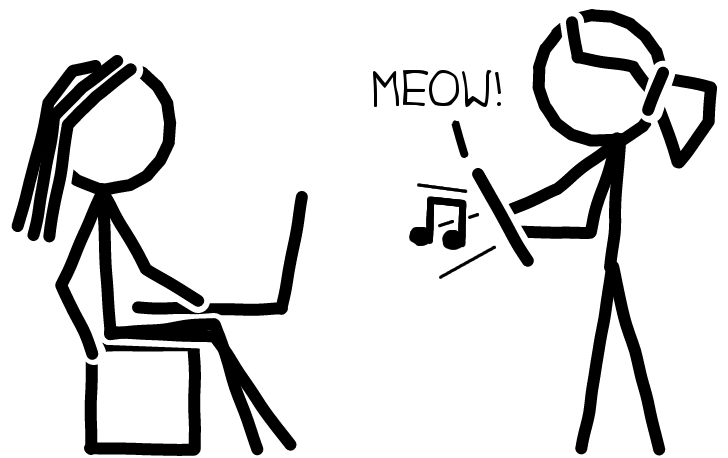
\includegraphics[width=.4\textwidth]{graphics/done.png}
\end{center}

\section{Prepare}

\begin{enumerate}
  \item Extract \textbf{StartGamedev} and open the text editor using the \texttt{open-editor} file.
  \item Read the tasks, type the code (\textit{source code}) and test the results.
\end{enumerate}

\section{Meow game app}

\subsection{Interactive sound}

\textbf{Type in} the following code, save it and test it:

\lstinputlisting{code/1all1.lua}

The code in \texttt{love.load()} loads a sound file and \texttt{love.mousepressed()} plays it when a mouse button is pressed or the touchscreen is touched.

\subsection{Interactive image}

\textbf{Insert} the loading of two images into \texttt{love.load()}:

\lstinputlisting{code/1load2en.lua}

\textbf{Add} the following two functions to your code:

\lstinputlisting{code/1add2en.lua}

\texttt{love.update()} calculates, which of the images is the current one. \texttt{love.draw()} draws it. Both functions work 60 times per second. The image doesn't quite fit but we will take care of that later.

\subsection{Random meow sounds}

\textbf{Add} the following list (or table) of sounds to \texttt{love.load()}:

\lstinputlisting{code/1load3en.lua}

\textbf{Replace} the content of \texttt{love.update()} with code, which uses the sound list:

\lstinputlisting{code/1update3en.lua}

\textbf{Replace} the content of \texttt{love.mousepressed()} with code which plays random sounds:

\lstinputlisting{code/1mousepressed3en.lua}

\subsection{Adapt to different screens}

\textbf{Add} calculations of the relations between image and window size to \texttt{love.load()}:

\lstinputlisting{code/1load4.lua}

\textbf{Add} scaling parameters to the \texttt{love.graphics.draw()} function call in \texttt{love.draw()}:

\lstinputlisting{code/1draw4en.lua}

The image fits to the screen size this way, since mobile phones/tablets only have one resolution. This is not optimal but a simple solution for the start.

\subsection{Android port} \label{androidport}

You can put own graphics (drawn on the computer or on paper) and sounds into your meow game app and change the app icon.

We recommend to code the ``back'' button to close the Android app:

\lstinputlisting{code/1keypressed5.lua}

To make the app playable on Android, a zip archive of the game must be made, renamed to \texttt{game.love} and put into the \texttt{StartGamedev} directory. Then use the \texttt{make-apk} script. The resulting \texttt{game.apk} must then be put on the mobile phone/tablet and installed there.

\newpage

\section{Cat and mouse game app}

\subsection{Image and sound}

\textbf{Type in} the following code (without \texttt{-{}- comments}), save it and test it:

\lstinputlisting{code/2all1en.lua}

The code in \texttt{love.load()} changes the screen resolution, loads the images and music, sets position variables and plays the msuic. \texttt{love.draw()} draws the images, 60 times per second. They don't quite fit but we will take care of that later.

\newpage

\subsection{Automatic and interactive movement}

\textbf{Add} mouse click position variables and sounds to \texttt{love.load()}:

\lstinputlisting{code/2load2en.lua}

\textbf{Add} the following three functions to your code:

\lstinputlisting{code/2add2en.lua}

The \texttt{distance()} function calculates the distance between two dots thanks to the Pythagoras' theorem or the formula $c = \sqrt{a^2 + b^2}$.

\texttt{love.update()}
\begin{enumerate*}
  \item Moves the mouse,
  \item Puts the mouse back, after it crosses the right border or
  \item when cat and mouse touch,
  \item moves the cat
\end{enumerate*}

The code in \texttt{love.mousepressed()} changes the \texttt{clickX} and \texttt{clickY} variables each time a mouse button is pressed or the touchscreen is touched.

\newpage

\subsection{Screen size}

\textbf{Add} calculations of the relations between image and window size to \texttt{love.load()}:

\lstinputlisting{code/2load3.lua}

\textbf{Add} scaling parameters to the \texttt{love.graphics.draw()} function call in \texttt{love.draw()}:

\lstinputlisting{code/2draw3en.lua}

\textbf{Replace} the variable assignments in \texttt{love.mousepressed()}, to project from the screen:

\lstinputlisting{code/2mousepressed3en.lua}

\subsection{Score and time}

\textbf{Add} image sizes, font configuration, time and score to \texttt{love.load()}:

\lstinputlisting{code/2load4en.lua}

\textbf{Add} time calculation to \texttt{love.update()}:

\lstinputlisting{code/2update4aen.lua}

\textbf{Add} a score counter to the \texttt{if} block in \texttt{love.update()} which reacts to cat and mouse touching:

\lstinputlisting{code/2update4ben.lua}

\textbf{Add} displaying time and score to \texttt{love.draw()}:

\lstinputlisting{code/2draw4en.lua}

You should put the content of \texttt{love.update()} into a \colorbox{lightgray}{\texttt{if time > 0 then ... end}} block to stop the game after the time runs out. You can use a similar block in \texttt{love.draw()} to display a ``Game Over!'' message.

\newpage

\section{Matrix music DJ app}

\textbf{Type in} the following code (without \texttt{-{}- comments}), save it and test it:

\lstinputlisting{code/3all1en.lua}

The code makes intense use of tables/lists and \texttt{for} loops as well as calculations, which might need a bit more time to be understood.

\end{document}
